\documentclass[11pt,a4paper]{article}
\usepackage[T1]{fontenc}
\usepackage{lmodern}
\usepackage{amsmath,amssymb,amsthm,mathtools}
\usepackage{booktabs,tabularx,array,graphicx}
\usepackage{float}
\usepackage{tikz}
\usetikzlibrary{arrows.meta,positioning,calc,fit,shapes.geometric}
\usepackage{geometry}
\usepackage{microtype}
\usepackage{setspace}
\usepackage{natbib}
\usepackage{hyperref}
\geometry{margin=1in}
\setstretch{1.12}
\hypersetup{colorlinks=true,linkcolor=blue,citecolor=blue,urlcolor=blue}
\newtheorem{theorem}{Theorem}
\newtheorem{proposition}[theorem]{Proposition}
\newtheorem{lemma}[theorem]{Lemma}
\newtheorem{corollary}[theorem]{Corollary}
\theoremstyle{remark}\newtheorem{remark}[theorem]{Remark}
\newcommand{\SW}{\mathrm{SW}}\newcommand{\SU}{\mathrm{SU}}\newcommand{\IS}{\mathrm{IS}}
\newcommand{\N}{\mathrm{N}}\newcommand{\F}{\mathrm{F}}
\newcommand{\loss}{\mathcal L}\newcommand{\vect}[1]{\boldsymbol{#1}}
\title{Endogenous Product Design and Participation in\\ International Compatibility Agreements}
\author{Review working draft---author details withheld}
\date{22 October 2026\quad |\quad Stage 13 integrated working draft\quad |\quad \textbf{Not for submission}}
\begin{document}
\maketitle
\begin{abstract}
Can privately optimal product redesign overturn governments' incentives to join an international compatibility agreement? We develop a three-country model in which governments choose bilateral or multilateral compatibility arrangements, firms subsequently choose residual product characteristics in Nash equilibrium, and production takes place in Cournot markets with network effects. Holding the governmental accession protocol fixed, we compare endogenous design with a benchmark that freezes firms' characteristics at their no-agreement levels. A national-welfare decomposition isolates the direct gain from an agreement and the induced loss arising from private redesign. Under explicit sufficient conditions the latter reverses both an initial member's participation incentive and an outsider's accession incentive. A certified nonempty open set of primitive parameters supports a stronger equilibrium contrast: positive-depth multilateral coordination is chosen with fixed design but the sequential-accession game remains fragmented with endogenous design. Direct multilateral agreement can nevertheless improve every country's welfare. The fragmentation result is therefore conditional on an inherited-depth accession procedure, not an impossibility of cooperation under unrestricted bargaining. Adjustment costs and network intensity delineate additional, explicitly limited boundaries. We distinguish this design-incidence mechanism from previously established results on product-standard coalitions and regulatory cooperation.
\end{abstract}
\noindent\textbf{Keywords:} compatibility standards; endogenous product differentiation; national welfare; coalition accession; network externalities; Cournot competition; institutional commitment.\\
\textbf{JEL:} F13, F15, L13, L15, D62, C72.

\section{Introduction}
A common compatibility standard can increase the value of consumption across jurisdictions. Yet the policy that appears desirable with a fixed configuration of products need not remain politically acceptable after firms respond. Product developers can change the attributes left outside the standard, and those changes affect a government's domestic consumers and the profits of its firms in every destination market. A national government consequently evaluates a different payoff from the one implicit in an engineering-only comparison of compatible products.

We examine a question at the boundary of industrial organization and public economic theory: \emph{Can the noncooperative redesign of products, by itself, reverse national consent to a compatibility agreement when the government's menu of agreements has not changed?} A second question asks which part of the resulting noncooperation reflects private incentives, and which reflects the institutional route through which countries attempt to cooperate.

The distinction is subtle. Existing research has already shown that regional standard-setting can prevent globally attractive harmonization \citep{Takarada2020,Kawabata2021}; other work combines national product regulation with firms' endogenous attribute choices \citep{Grossman2021}. Endogenous compatibility choice and private veto effects are also familiar in network industries \citep{Buccella2023,Cheng2025}. Our contribution is \emph{not} the generic existence of incomplete standards coalitions, nor the idea that companies adapt products in response to regulation. We isolate an additional, model-specific \emph{national-incidence channel}: firms' residual-design Nash responses subtract from the direct national benefit of compatibility, and the subtraction can change the sign of government participation inequalities under precisely the same government accession rules.

To identify this channel, we hold constant demand, country welfare objectives, the possible compatibility link patterns, and the sequence of governmental offers. Only firms' subsequent design behavior differs across our principal comparison. We derive a transparent local decomposition,
\begin{equation}\label{eq:introheadline}
\left.\frac{\partial m_{\F}(g)}{\partial g}\right|_{g=0}=D>0,\qquad
\left.\frac{\partial m_{\N}(g)}{\partial g}\right|_{g=0}=D-\loss<0,
\end{equation}
where $m$ is a prospective bilateral member's national welfare, $D$ is the direct effect at fixed design, and $\loss$ is the incidence of firms' equilibrium redesign on domestic consumer surplus and home-firm worldwide profits. The private first-order condition does not set these national effects to zero. Exchangeability across three countries then transmits the same sign reversal to the outsider's incentive to join an existing bilateral arrangement.

A second result moves beyond a derivative at one point. Using independently checked equilibrium equations and existing rigorous interval certificates, we identify a nonempty \emph{open neighborhood} of primitive parameters in which all positive-depth proposals fail under the specified inherited-depth, bilateral-first procedure when product design is endogenous; with the same primitives and governmental procedure, freezing residual design yields an accepted, government-preferred multilateral agreement. A positive-depth direct grand agreement would nevertheless raise welfare in all three countries under endogenous design. Hence the failure is neither an engineering impossibility nor a general claim of coalition-proof fragmentation.

The institutional restriction is deliberate. The initial bilateral proposal specifies a compatibility depth that a later entrant may accept or reject but cannot revise in the same accession round. This separates accession to an existing specification from negotiation of a newly specified multilateral interface. Larger standard-setting committees can face distributive bargaining frictions \citep{Simcoe2012}; nevertheless, the model \emph{does not} prove that this procedure is endogenously optimal, that technical specifications cannot be amended in practice, or that direct multilateral negotiation is unavailable in every standards organization. The direct-proposal counterfactual is used expressly to reveal this limitation.

Sections~\ref{sec:model}--\ref{sec:global} develop the model, private Nash incidence, and all-depth result. Section~\ref{sec:institution} isolates the effect of the accession procedure, Section~\ref{sec:boundaries} reports restricted boundaries, and the Appendix supplies proof and computational details.

\section{Economic environment and the accession protocol}\label{sec:model}
\subsection{Three countries, compatibility, and residual design}
There are three symmetric countries $A,B,C$, each with one firm. All three firms sell in each of three identical segmented national markets. Each firm chooses the degree $x_i\in[0,1]$ of residual product similarity, namely how much of the product architecture outside the publicly harmonized interface is left common across goods. Equivalently, $1-x_i$ measures the intensity of \emph{costly private differentiation}; it is the reverse scale of this same choice, not a second attribute. Firms can save development costs by raising $x_i$, but doing so changes product substitution and their Cournot profits. The compatibility arrangement is a separate government choice: $g$ specifies the publicly agreed technical depth, whereas $x_i$ describes privately chosen differentiation in the residual design space. This intentionally parsimonious linear relationship between firms' characteristics and pairwise similarity is a modeling assumption, not a universal engineering identity.

Let $g\in[0,1]$ denote the proposed depth of common compatibility and write $H$ for the country-link matrix: $H_{ii}=1$ and $H_{ij}=0$ under fragmentation $\SW$, $H_{AB}=H_{BA}=g$ with other off-diagonal entries zero under bilateral compatibility $\SU$, and $H_{ij}=g$ for every $i\ne j$ under integrated compatibility $\IS$. Define $X_{ii}=1$ and $X_{ij}=(x_i+x_j)/2$ for $i\ne j$. The cross-product matrix and fulfilled-expectations Cournot matrix are
\begin{equation}\label{eq:matrices}
B=\rho H+(1-\rho)X,\qquad M=I+B-\eta H,
\end{equation}
where $\rho$ is the weight placed on the government-specified compatibility component and $\eta$ is the strength of fulfilled network effects. In particular, $g$, $x_i$, and $\rho$ play different roles; they must not be interpreted as interchangeable measures of product differentiation.

For one destination market, an integrable quadratic consumer payoff yielding the inverse demands can be written, for fixed network expectations $\bar{q}$, as
\begin{equation}\label{eq:consumer}
U(q;\bar q)=(c+d)\vect{1}^{\top}q-\tfrac12q^{\top}Bq+\eta q^{\top}H\bar q,\qquad
p=(c+d)\vect{1}-Bq+\eta H\bar q.
\end{equation}
The matrix $B$ is symmetric and positive semidefinite on the full strategy cube for the maintained $0\le\rho\le1$; Appendix~\ref{app:regularity} proves this from the matrices' vertices. At the benchmark $0<\eta<\rho<1$ and the sufficient full-cube Rosen bound holds, delivering positive Cournot quantities and a unique private-design Nash continuation (Appendix~\ref{app:regularity}). Consumers and firms take network expectations as fixed during a unilateral quantity deviation; expectations are fulfilled at equilibrium. Every firm's constant marginal production cost is $c$ and $d>0$ is the net-demand intercept.

In the baseline, firm $i$ bears a one-time design cost
\begin{equation}\label{eq:cost}
K_i(x_i)=\tfrac{\kappa}{2}(1-x_i)^2,\qquad\kappa>0.
\end{equation}
The quadratic cost is the expense of developing proprietary differentiation $1-x_i$: as $x_i$ increases toward one, firms economize on differentiation effort while their products become more alike. Hence the Nash redesign response includes a genuine private cost-saving incentive. The optional curvature $\lambda(x_i-z)^2/2$ is introduced only in Section~\ref{sec:boundaries}; it is not part of the baseline result. Because each firm sells in three identical markets, its worldwide operating profit is $3q_i^2$ in the fulfilled interior Cournot equilibrium derived below. The resulting net profit and each country's national welfare are
\begin{equation}\label{eq:welfare}
\Pi_i=3q_i^2-K_i(x_i),\qquad CS=\tfrac12q^{\top}Bq,\qquad W_i=CS+\Pi_i.
\end{equation}
$CS$ is the consumer surplus of the country's own representative destination market, whereas $\Pi_i$ includes its resident firm's profits in \emph{all three} markets. Symmetry of destination markets justifies the same $CS$ expression for each country, not adding the surplus of three countries to national welfare. The separation between domestic consumers and worldwide firm earnings is essential to the result.

\subsection{Timing, government choices, and the consent inequalities}
The game is solved by backward induction. The policy stage specifies $H$ and the depth $g$; firms then choose $x_i$ simultaneously and noncooperatively; finally they choose Cournot quantities in their destination markets. We assume unique positive-output continuation equilibria when deriving differentiable reduced-form payoffs and explicitly restrict global claims to the certified region.

At the policy level, country $A$ initiates an $AB$ bilateral proposal at depth $g\in[0,1]$. Country $B$ chooses whether to accept, anticipating the specified later accession opportunity. Country $C$ may then join at the \emph{same inherited depth}; accession requires the approval of $C$ and incumbents. Accession approval is implemented as a sequence of perfectly observed yes/no decisions by C, A, and B, each conditional on preceding approvals. Every government is required to vote yes when its eventual payoff is unchanged, including at off-path histories and when its ballot would otherwise be nonpivotal; a strict preference for rejection is needed for a veto. Depth is set at the initial proposal and is not reoptimized upon accession within this game. Country $A$ selects its initial offer to maximize the welfare resulting from the actual continuation game. A later direct three-country negotiation is not part of this baseline protocol.

For policy regime $r\in\{\SW,\SU,\IS\}$ write $x^r(g)$ for the actual firm Nash equilibrium and $W^r(g)$ for the resulting national welfare. Define, with symmetry,
\begin{align}\label{eq:payoffs}
s&=W_A^{\SW}=W_B^{\SW}=W_C^{\SW},\nonumber\\
m(g)&=W_A^{\SU}=W_B^{\SU},\qquad o(g)=W_C^{\SU},\nonumber\\
i(g)&=W_A^{\IS}=W_B^{\IS}=W_C^{\IS}.
\end{align}
At $g=0$, the regimes coincide, so $m(0)=o(0)=i(0)=s$. The inherited-depth regime rules, including the first member's anticipation of a later accession vote, are
\begin{align}\label{eq:consent}
\IS\text{ at }g &: \quad i(g)\ge\max\{s,m(g),o(g)\},\\
\SU\text{ at }g &: \quad m(g)\ge s\text{ and at least one enlargement vote fails},\nonumber\\
\SW &: \quad\text{otherwise}.\nonumber
\end{align}
Indeed, after B accepts an AB offer, C compares $i(g)$ with $o(g)$, and the incumbent voters compare $i(g)$ with $m(g)$; B anticipates this accession subgame and compares either its final $i(g)$ or $m(g)$ with $s$. Thus unanimous enlargement followed by initial acceptance occurs exactly when $i(g)\ge\max\{s,m(g),o(g)\}$. The tie convention applies at every subgame, not just on the equilibrium path. These conditions describe the baseline extensive-form outcome; they are \emph{not} the core of the unrestricted coalition-formation game. In particular, positive $i(g)-s$ alone never proves acceptance under inherited-depth enlargement.

Figure~\ref{fig:timing} separates the governmental proposal and voting tree from the firm and market continuations used to evaluate each terminal regime. The latter are solved first when computing the former by backward induction.


\begin{figure}[tbp]
\centering
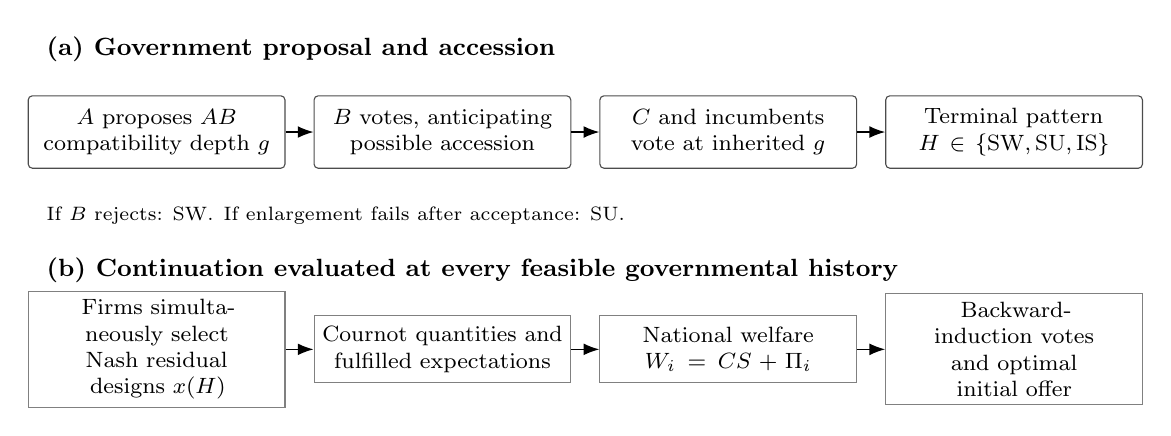
\begin{tikzpicture}[x=1cm,y=1cm,>=Latex,
    gov/.style={draw=black!70,rounded corners=1.5pt,align=center,
      text width=3.05cm,minimum height=0.92cm,font=\footnotesize,inner sep=3pt},
    econ/.style={draw=black!50,align=center,text width=3.05cm,
      minimum height=0.85cm,font=\footnotesize,inner sep=3pt},
    arrow/.style={-{Latex[length=2mm]},line width=.45pt}]
\node[anchor=west,font=\small\bfseries] at (0,1.05) {(a) Government proposal and accession};
\node[gov] (a) at (1.52,0) {$A$ proposes $AB$\\compatibility depth $g$};
\node[gov] (b) at (5.15,0) {$B$ votes, anticipating\\possible accession};
\node[gov] (c) at (8.78,0) {$C$ and incumbents\\vote at inherited $g$};
\node[gov] (h) at (12.41,0) {Terminal pattern\\$H\in\{\SW,\SU,\IS\}$};
\draw[arrow] (a.east) -- (b.west);
\draw[arrow] (b.east) -- (c.west);
\draw[arrow] (c.east) -- (h.west);
\node[font=\scriptsize,anchor=west] at (0,-1.06) {If $B$ rejects: $\SW$. If enlargement fails after acceptance: $\SU$.};
\node[anchor=west,font=\small\bfseries] at (0,-1.75) {(b) Continuation evaluated at every feasible governmental history};
\node[econ] (x) at (1.52,-2.76) {Firms simultaneously select\\Nash residual designs $x(H)$};
\node[econ] (q) at (5.15,-2.76) {Cournot quantities and\\fulfilled expectations};
\node[econ] (w) at (8.78,-2.76) {National welfare\\$W_i=CS+\Pi_i$};
\node[econ] (v) at (12.41,-2.76) {Backward-induction votes\\and optimal initial offer};
\draw[arrow] (x.east) -- (q.west);
\draw[arrow] (q.east) -- (w.west);
\draw[arrow] (w.east) -- (v.west);
\end{tikzpicture}
\caption{Game timing and the role of continuation payoffs. Governments specify a possible compatibility pattern and depth; for each contemplated terminal pattern firms select residual designs before Cournot competition. Governments anticipate these continuation payoffs when voting. The baseline does not permit renegotiation of $g$ at accession.}
\label{fig:timing}
\end{figure}

\section{Cournot equilibrium and private design response}\label{sec:equilibrium}
\subsection{Market-stage equilibrium and the no-agreement reference}
Since $B_{ii}=1$, firm $i$'s Cournot first-order condition at fixed expectations is $p_i-c=q_i$. Imposing fulfilled expectations $\bar q=q$ gives
\begin{equation}\label{eq:cournot}
M q=d\vect{1},\qquad q=d M^{-1}\vect{1},
\end{equation}
provided $M$ is invertible and $q\gg0$. The expression defines outputs conditional on policy $H$ and design $x$. It is the interior continuation formula, not by itself a global design-equilibrium certificate. For $E_j=M_{x_j}$, unilateral private-design differentiation gives $q_{x_j}=-M^{-1}E_jq$ and $F_i=6q_i(q_{x_i})_i+\kappa(1-x_i)$. This is the own-firm FOC holding all rival designs fixed; the full-cube Nash uniqueness and boundary-deviation conditions are supplied in Appendix~\ref{app:regularity}.

Write the useful abbreviations
\begin{equation}\label{eq:abbrev}
\alpha=2-\eta,\quad\beta=1-\rho,\quad\delta=\rho-\eta,\quad
t=\beta z,\quad P=\alpha-t,\quad L=\alpha+2t.
\end{equation}
At fragmentation the symmetric interior design Nash $z$ obeys
\begin{equation}\label{eq:root}
\kappa(1-z)=\frac{6\beta\alpha d^2}{(\alpha-t)L^3},\qquad t=\beta z,\qquad q_0=\frac dL.
\end{equation}
The solution on the certified branch has $0<z<1$ and $P,L>0$. The derivation uses the \emph{unilateral} firm-design first-order condition; treating the firms as a common social planner would yield a different equation.

\subsection{The implicit Nash response rather than a planner response}
Let $F_i(x;H)=\partial\Pi_i(x;H)/\partial x_i$ be firm $i$'s own design derivative, already anticipating the quantity equilibrium in \eqref{eq:cournot}. The private Nash system is
\begin{equation}\label{eq:designFOC}
F_i(x;H)=0\quad (i=A,B,C).
\end{equation}
Where the full $3\times3$ Jacobian $J=\partial F/\partial x$ is nonsingular, the equilibrium design response to policy depth is
\begin{equation}\label{eq:implicit}
\frac{dx}{dg}=-J^{-1}\frac{\partial F}{\partial g}.
\end{equation}
This response incorporates the strategic adjustment of rival firms. It cannot be replaced by three independent optimizations holding their competitors' designs fixed. Similarly, each firm's private FOC annihilates the derivative of \emph{its own} profit with respect to \emph{its own} chosen design, but neither the effect on domestic consumers nor the effect of competitors' designs on its worldwide profit. This distinction generates our main incidence term.

\section{The national-incidence mechanism}\label{sec:mechanism}
\subsection{Symmetry turns one edge into an accession constraint}
For the derivative analysis, allow the three compatibility edges $e_{AB}$, $e_{AC}$, $e_{BC}$ to vary separately near zero. The firm continuation and national reduced payoffs inherit the permutation symmetry of the primitive game.
\begin{lemma}[Edge incidence]\label{lem:edges}
Assume differentiable, unique symmetric firm continuations at fragmentation. There exist numbers $\mu$ and $\nu$ such that a country's marginal welfare response to an incident compatibility edge is $\mu$, and its response to the remaining nonincident edge is $\nu$. Consequently,
\begin{equation}\label{eq:edges}
m'(0)=\mu,\quad o'(0)=\nu,\quad i'(0)=2\mu+\nu,\quad
[i-o]'(0)=2\mu,\quad [i-m]'(0)=\mu+\nu.
\end{equation}
The identities apply separately under endogenous and frozen residual design.
\end{lemma}
\begin{proof}
Differentiate each country's reduced welfare with respect to the three independently variable edges at zero. Permuting country labels leaves the game invariant. For any country, the two incident edges therefore have a common coefficient $\mu$, and the third edge has coefficient $\nu$. A bilateral $AB$ link activates one edge; a common-depth grand standard activates all three. Taking directional derivatives and subtracting gives \eqref{eq:edges}.
\end{proof}

The lemma is a symmetry accounting identity, not a new economic discovery. Its use here is to show exactly why a member's marginal incentive also determines the outsider's \emph{accession} comparison. The incumbent and outsider votes are distinct government comparisons, but their first-order effects are linked by the three-country structure.

\subsection{What private redesign subtracts from national welfare}
Define the \emph{frozen-design} counterfactual by keeping every $x_i=z$, its actual no-agreement Nash value, at all positive-depth policy histories. Firms still compete in the Cournot market, governments still optimize the initial depth, and the accession and rejection rules are unchanged. Let subscript $\F$ denote these payoffs and $\N$ the fully endogenous design payoffs. At $g=0$ both regimes coincide.

An $AB$ link at fixed $x=z$ yields the bilateral-member national welfare slope
\begin{equation}\label{eq:D}
D\equiv\mu_{\F}=
\frac{\rho d^2}{L^2}-\frac{\delta d^2}{L^3}
\left(2(1+2t)+\frac{6\alpha}{P}\right).
\end{equation}
This combines a direct compatibility-related consumer gain with the effects of output adjustment on consumer surplus and on the home firm's profits. The outsider's frozen-design response is
\begin{equation}\label{eq:nuF}
\nu_{\F}=\frac{\rho d^2}{L^2}-\frac{2\delta d^2(1+2t)}{L^3}
+\frac{12\delta d^2t}{PL^3}.
\end{equation}
With endogenous design, symmetry of $AB$ implies two relevant slopes, $u'=dx_A^{\SU}/dg|_0=dx_B^{\SU}/dg|_0$ and $v'=dx_C^{\SU}/dg|_0$, determined by \eqref{eq:implicit}.

The derivative of $A$'s \emph{national welfare}, evaluated at the no-agreement private Nash, satisfies
\begin{equation}\label{eq:Wgrad}
\partial_{x_A}W_A=-C,\qquad
\partial_{x_B}W_A=\partial_{x_C}W_A=-(C+V),
\end{equation}
where
\begin{equation}\label{eq:CV}
C=\frac{\beta d^2(\eta+2t)}{L^3},\qquad
V=\frac{3\beta d^2(\alpha-2t)}{PL^3}.
\end{equation}
Here $C$ summarizes the consumer-side incidence, while $V$ captures the incremental worldwide home-profit response to \emph{other firms'} choices. Neither should be removed by invoking firm $A$'s own-profit FOC.

\begin{lemma}[National-welfare incidence of noncooperative design]\label{lem:incidence}
Under regular interior firm design Nash and the maintained primitives, the endogenous bilateral-member derivative is
\begin{equation}\label{eq:loss}
\mu_{\N}=D-\loss,\qquad
\loss\equiv C(2u'+v')+V(u'+v').
\end{equation}
In particular, $C,V,u',v'>0$ implies $\loss>0$. If $0<D<\loss$, a member gains from a marginal compatibility link under frozen design but loses after noncooperative redesign.
\end{lemma}
\begin{proof}
Apply the chain rule to $W_A(g,x^\SU(g))$ at zero. Its fixed-design part is $D$ by \eqref{eq:D}. The Nash-adjustment part is $\partial_x W_A\cdot(u',u',v')$, which by \eqref{eq:Wgrad} equals $-C(2u'+v')-V(u'+v')$. This establishes \eqref{eq:loss}. Positivity yields the final inequality. The derivative of the own optimized \emph{private profit} with respect to $x_A$ vanishes, but its domestic consumer effect and the response to rivals' designs do not; omitting the $V$ term changes the conclusion and is incorrect.
\end{proof}

\paragraph{Economic interpretation.}
There is no general welfare envelope theorem for a government when firms privately optimize product positions. Standardization changes the privately desirable residual characteristics. A firm has no incentive to internalize every resident consumer's lost surplus, nor the effect of competitors' adjustments on its export profits. A sufficiently strong induced response therefore destroys a government gain that would have been present if product attributes were constrained. Our analytical innovation is the \emph{incidence and policy comparison within this particular two-level game}, not the abstract chain rule $D-\loss$ alone.

Figure~\ref{fig:mechanism} summarizes the identifying experiment: no policy primitive or government voting rule changes between the frozen and endogenous-design cases.


\begin{figure}[tbp]
\centering
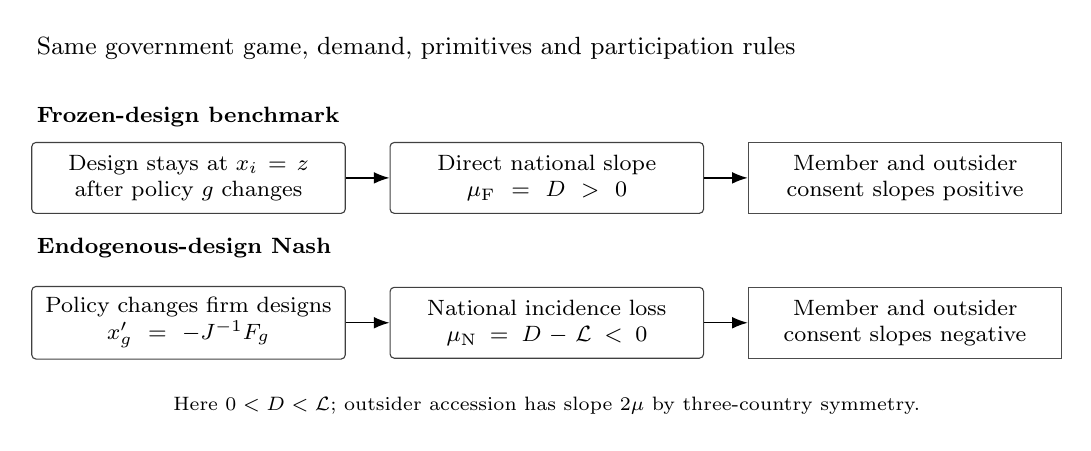
\begin{tikzpicture}[x=1cm,y=1cm,>=Latex,
    mech/.style={draw=black!75,rounded corners=1.5pt,align=center,font=\footnotesize,
       minimum height=0.9cm,text width=3.7cm,inner sep=4pt},
    answer/.style={draw=black!70,align=center,font=\footnotesize,
       minimum height=0.9cm,text width=3.7cm,inner sep=4pt},
    arrow/.style={-{Latex[length=2mm]},line width=.5pt}]
\node[font=\small,anchor=west] at (-0.05,1.45) {Same government game, demand, primitives and participation rules};
\node[font=\footnotesize\bfseries,anchor=west] at (-0.05,0.57) {Frozen-design benchmark};
\node[mech] (f1) at (2.0,-0.20) {Design stays at $x_i=z$\\after policy $g$ changes};
\node[mech] (f2) at (6.55,-0.20) {Direct national slope\\$\mu_{\F}=D>0$};
\node[answer] (f3) at (11.1,-0.20) {Member and outsider\\consent slopes positive};
\draw[arrow] (f1.east) -- (f2.west);
\draw[arrow] (f2.east) -- (f3.west);
\node[font=\footnotesize\bfseries,anchor=west] at (-0.05,-1.09) {Endogenous-design Nash};
\node[mech] (n1) at (2.0,-2.04) {Policy changes firm designs\\$x'_g=-J^{-1}F_g$};
\node[mech] (n2) at (6.55,-2.04) {National incidence loss\\$\mu_{\N}=D-\mathcal L<0$};
\node[answer] (n3) at (11.1,-2.04) {Member and outsider\\consent slopes negative};
\draw[arrow] (n1.east) -- (n2.west);
\draw[arrow] (n2.east) -- (n3.west);
\node[font=\scriptsize,align=center] at (6.55,-3.09)
 {Here $0<D<\mathcal L$; outsider accession has slope $2\mu$ by three-country symmetry.};
\end{tikzpicture}
\caption{Controlled causal comparison at the no-agreement boundary. Private redesign affects both domestic consumer surplus and the home firm's worldwide profits; the private firm's own first-order condition does not eliminate this national incidence. The diagram summarizes the \emph{local} sign result, not a general theorem of agreement failure under every bargaining protocol.}
\label{fig:mechanism}
\end{figure}

\section{Main result: private redesign reverses governmental consent}\label{sec:global}
\begin{theorem}[Local controlled participation reversal]\label{thm:local}
Suppose the firm continuation is regular, unique, interior, and continuously differentiable near fragmentation, and suppose the primitive parameters imply $\beta>0$, $\rho>\eta$, $C,V,u',v'>0$ and
\begin{equation}\label{eq:conditions}
0<D<\loss,\qquad \nu_{\N}>-2\mu_{\N},\qquad \nu_{\F}>-D.
\end{equation}
For every sufficiently small $g>0$, (a) with frozen design the inherited-depth procedure has affirmative bilateral-member and outsider-accession votes, and an acceptable integrated agreement strictly improves on fragmentation; (b) with endogenous design, the bilateral-member and outsider-accession conditions fail while the hypothetical integrated allocation at the same depth strictly Pareto-improves on fragmentation. The statement is local in $g$; it does not alone establish the government-optimal regime over all depths.
\end{theorem}
\begin{proof}
By Lemma~\ref{lem:incidence}, $\mu_{\F}=D>0$ but $\mu_{\N}=D-\loss<0$. Lemma~\ref{lem:edges} gives the frozen outsider accession slope $[i_{\F}-o_{\F}]'(0)=2D>0$ and incumbent widening slope $[i_{\F}-m_{\F}]'(0)=D+\nu_{\F}>0$. The frozen grand benefit slope is $2D+\nu_{\F}>0$. In the endogenous game, $m_{\N}'(0)=\mu_{\N}<0$ and $[i_{\N}-o_{\N}]'(0)=2\mu_{\N}<0$, whereas $i_{\N}'(0)=2\mu_{\N}+\nu_{\N}>0$. Each compared level gap is zero at $g=0$. Strict derivative inequalities and differentiability therefore imply the specified level inequalities for all sufficiently small positive $g$. The government's comparison in \eqref{eq:consent} then produces the stated local voting outcomes.
\end{proof}

Both treatments use the same governmental strategies and payoffs; only the post-agreement private Nash response differs. Section~\ref{sec:institution} shows why the failure does not extend to direct multilateral proposals.

\begin{theorem}[An open primitive region with different government-optimal outcomes]\label{thm:open}
There exists a nonempty open neighborhood $\mathcal U$ of
\begin{equation}\label{eq:theta}
\theta_0=(d,\eta,\rho,\kappa)=\left(1,\frac{379}{500},\frac9{10},\frac{1701}{2000}\right)
\end{equation}
in the four-dimensional baseline primitive parameter space such that the following hold in the maintained inherited-depth game:
\begin{enumerate}
\item With endogenous firm design, every strictly positive-depth proposal fails the original accession procedure; the government-optimal equilibrium regime is fragmentation $\SW$.
\item With all residual designs fixed at their \emph{same} no-agreement Nash $z$, a strictly positive-depth integrated agreement is approved and yields a higher initiating-country payoff than any terminal bilateral arrangement or fragmentation; hence a government-optimal positive $\IS$ proposal exists.
\item For these primitives, some hypothetical direct integrated agreement under endogenous design strictly improves the national welfare of all three countries relative to $\SW$.
\end{enumerate}
This does not assert an explicit radius for $\mathcal U$, an all-parameter global classification, or coalition-proof fragmentation.
\end{theorem}
\begin{proof}[Proof architecture and certified bounds]
At $\theta_0$, the reproducible all-depth interval proof described in Appendix~\ref{app:interval} establishes, for $g\in[0,1]$, strict derivative \emph{upper} bounds
\begin{equation}\label{eq:cert}
\frac{dm_{\N}}{dg}<-0.0079701929973,\qquad
\frac{d(i_{\N}-o_{\N})}{dg}<-0.0150388833377.
\end{equation}
The underlying checks include the unique full-firm Nash continuation, positive quantities, regularity and enclosure of the derivative along the full policy-depth interval; they are not merely a local FOC calculation. Integrating from $g=0$, where all regime welfare levels coincide, yields $m_{\N}(g)<s$ and $i_{\N}(g)<o_{\N}(g)$ at every $g>0$. Thus neither an accepted $\SU$ nor an enlargement to $\IS$ survives the original voting conditions; optimizing over the full depth menu returns $\SW$.

For the frozen-design game, the previously certified all-depth bilateral payoff bound and the strictly feasible integrated candidate at $g=1/20$ give
\begin{equation}\label{eq:frozenCert}
 i_{\F}(1/20)>2.4413970373,
\quad s<2.4220784218,
\quad\sup_{0\le g\le1}m_{\F}(g)<2.4235735642,
\end{equation}
while $i_{\F}(1/20)>o_{\F}(1/20)$ and $i_{\F}(1/20)>m_{\F}(1/20)$ strictly. The candidate is accepted, beats $\SW$, and beats the entire terminal bilateral payoff envelope, so an optimal accepted positive-depth integrated offer exists. Separately the actual endogenous integrated outcome at $g=1/20$ satisfies $i_{\N}(1/20)-s>0.0169346278736$.

The all-depth strict inequalities, positive-output margins and uniform full-cube equilibrium-uniqueness/regularity margins survive under sufficiently small primitive perturbations. A finite-cover implicit-function argument, continuity of derivatives on a compact depth interval, and the maximum theorem preserve strict negative endogenous slopes and the strict frozen integrated-versus-bilateral envelope gap. The local no-agreement and positive-depth inequalities thereby hold on some common \emph{open} neighborhood $\mathcal U$. The existence assertion is qualitative; no explicit primitive box is supplied. Appendix~\ref{app:interval} identifies the certified mathematical objects, interval algorithm, and immutable reproduction artifacts, which form part of the manuscript-facing proof package.
\end{proof}

The local inequality $0<D<\loss$ identifies the mechanism; the all-depth derivative certificate excludes any compensating inherited-depth proposal. Continuity extends the strict inequalities to an unquantified primitive neighborhood, not to other governmental agendas, demand classes, or country counts.

Table~\ref{tab:map} distinguishes the main reversal from the institutional and parameter-boundary results; it also records where the proofs are local, all-depth or restricted to a limiting family.


\begin{table}[tbp]
\centering\footnotesize
\caption{Hierarchy, proven domains, and limits of the results}\label{tab:map}
\renewcommand{\arraystretch}{1.22}
\begin{tabularx}{\linewidth}{@{}>{\raggedright\arraybackslash}p{.18\linewidth}>{\raggedright\arraybackslash}p{.34\linewidth}>{\raggedright\arraybackslash}X@{}}
\toprule
Result & Proven environment or condition & Inference and scope limit \\
\midrule
Local reversal & $0<D<\mathcal L$, regular design Nash; additional outsider slope conditions & Frozen design gives positive consent slopes; endogenous design reverses both. \emph{Local} in $g$. \\
Global regime & Certified all-depth inequalities at $\theta_0$ and a nonempty open primitive neighborhood & $\SW$ with design Nash versus government-optimal $\IS$ with frozen design. Specific inherited-depth protocol; not coalition-proof. \\
Direct-grand & $\mu_{\N}<0<2\mu_{\N}+\nu_{\N}$ & Direct $\IS$ can benefit all at the same small $g$; procedural boundary, not a general new coalition theorem. \\
Design costs & $\lambda_c\in(0.93538,0.93539)$ at $\theta_0$ & Unique \emph{local} consent cutoff; no global $\lambda$ regime classification. \\
Network intensity & $\rho=1$, $\eta=6/7$ cutoff and restricted $\rho<1$ strip & Exact global regimes on the design-inactive face; only restricted nearby endogenous extension. \\
\bottomrule
\end{tabularx}
\end{table}

\subsection{An interpretable numerical illustration}
At $\theta_0$ the no-agreement symmetric private design is $z\simeq0.7185927073$. We obtain $D\simeq0.0067679241$, $\loss\simeq0.0150697441$ and $\mu_{\N}\simeq-0.0083018200$. For the same policy depth $g=0.05$, all values below are \emph{national welfare differences} from the corresponding bilateral, outsider, or fragmentation alternatives. Table~\ref{tab:effects} uses an independently evaluated Cournot--design Nash continuation and illustrates magnitudes and signs; it does not replace the rigorous all-depth argument.
\begin{table}[ht]
\centering\small
\caption{Government welfare comparisons at $g=0.05$ (uncalibrated model units)}\label{tab:effects}
\begin{tabular}{lrrr}
\toprule
Firm-design treatment&$m-s$&$i-o$&$i-s$\\
\midrule
Frozen at original $z$&$+0.000272382$&$+0.000234617$&$+0.019318616$\\
Endogenous design Nash&$-0.000473474$&$-0.001246547$&$+0.016934628$\\
\bottomrule
\end{tabular}
\end{table}
Although $i_{\N}-s$ is positive at $g=0.05$, the bilateral-member and outsider-accession margins are negative. The welfare magnitudes are uncalibrated model units, not estimates of real-world agreement gains.

Figure~\ref{fig:phase} explores how the two private-design treatments differ on a common $(\kappa,\eta)$ slice. Each parameter pair uses its own fragmentation Nash design, with identical governmental voting rules in both panels. Acceptance windows can be narrow near $g=0$; the numerical search therefore combines logarithmic near-zero probes with brackets of observed consent-margin crossings and comparisons against computed bilateral payoff candidates. Blue cells identify accepted integrated offers that improve on the computed bilateral envelope. Gray cells mean \emph{no profitable accepted offer found in the search}, not proved absence of such an offer at every depth. Only the separately marked benchmark and the qualitative primitive neighborhood in Theorem~\ref{thm:open} carry the article's exact all-depth guarantee.

A bilateral agreement may pass consent votes at one depth but lose to an integrated offer at another depth. No proposer-optimal bilateral cell was identified on the $41\times41$ numerical slice; this does not establish a universal no-$\SU$ theorem. The plotted boundaries are exploratory rather than certified two-dimensional phase curves.

\begin{figure}[H]
\centering
\resizebox{0.98\linewidth}{!}{% Auto-generated numeric slice; not a certification of all parameter values.
\begingroup
\definecolor{mapSW}{RGB}{220,220,220}
\definecolor{mapSU}{RGB}{238,195,120}
\definecolor{mapIS}{RGB}{89,139,187}
\definecolor{mapUN}{RGB}{249,249,249}
\begin{tikzpicture}[x=7.05cm,y=5.2cm,>=Latex]
\begin{scope}[shift={(0.000,0)}]
\fill[mapSW] (0.0000000,0.0000000) rectangle (1.0000000,0.4390244);
\fill[mapSW] (0.0000000,0.4390244) rectangle (0.6585366,0.4634146);
\fill[mapIS] (0.6585366,0.4390244) rectangle (1.0000000,0.4634146);
\fill[mapIS] (0.0000000,0.4634146) rectangle (1.0000000,1.0000000);
\draw[black!80,line width=.45pt] (0,0) rectangle (1,1);
\node[anchor=south,font=\footnotesize\bfseries] at (.5,1.045) {(a) Frozen design};
\node[font=\small\bfseries] at (.48,.81) {IS};
\node[font=\small\bfseries] at (.51,.25) {SW};
\node[font=\footnotesize] at (.5,-.16) {Design cost $\kappa$};
\draw (0.000000,0)--(0.000000,-.013) node[below,font=\scriptsize]{0.70};
\draw (0.285714,0)--(0.285714,-.013) node[below,font=\scriptsize]{0.80};
\draw (0.571429,0)--(0.571429,-.013) node[below,font=\scriptsize]{0.90};
\draw (0.857143,0)--(0.857143,-.013) node[below,font=\scriptsize]{1.00};
\draw (0,0.000000)--(-.012,0.000000) node[left,font=\scriptsize]{0.742};
\draw (0,0.266667)--(-.012,0.266667) node[left,font=\scriptsize]{0.750};
\draw (0,0.533333)--(-.012,0.533333) node[left,font=\scriptsize]{0.758};
\draw (0,0.800000)--(-.012,0.800000) node[left,font=\scriptsize]{0.766};
\draw (0,1.000000)--(-.012,1.000000) node[left,font=\scriptsize]{0.772};
\node[star,star points=5,draw=black,fill=black,minimum size=5pt,inner sep=0pt] at (0.4300000,0.5333333) {};
\node[rotate=90,font=\footnotesize] at (-.23,.5) {Network effect $\eta$};
\end{scope}
\begin{scope}[shift={(1.130,0)}]
\fill[mapSW] (0.0000000,0.0000000) rectangle (1.0000000,0.5853659);
\fill[mapSW] (0.0000000,0.5853659) rectangle (0.6829268,0.6097561);
\fill[mapIS] (0.6829268,0.5853659) rectangle (1.0000000,0.6097561);
\fill[mapSW] (0.0000000,0.6097561) rectangle (0.4634146,0.6341463);
\fill[mapIS] (0.4634146,0.6097561) rectangle (1.0000000,0.6341463);
\fill[mapSW] (0.0000000,0.6341463) rectangle (0.2682927,0.6585366);
\fill[mapIS] (0.2682927,0.6341463) rectangle (1.0000000,0.6585366);
\fill[mapSW] (0.0000000,0.6585366) rectangle (0.1219512,0.6829268);
\fill[mapIS] (0.1219512,0.6585366) rectangle (1.0000000,0.6829268);
\fill[mapIS] (0.0000000,0.6829268) rectangle (1.0000000,1.0000000);
\draw[black!80,line width=.45pt] (0,0) rectangle (1,1);
\node[anchor=south,font=\footnotesize\bfseries] at (.5,1.045) {(b) Endogenous design};
\node[font=\small\bfseries] at (.48,.81) {IS};
\node[font=\small\bfseries] at (.51,.25) {SW};
\node[font=\footnotesize] at (.5,-.16) {Design cost $\kappa$};
\draw (0.000000,0)--(0.000000,-.013) node[below,font=\scriptsize]{0.70};
\draw (0.285714,0)--(0.285714,-.013) node[below,font=\scriptsize]{0.80};
\draw (0.571429,0)--(0.571429,-.013) node[below,font=\scriptsize]{0.90};
\draw (0.857143,0)--(0.857143,-.013) node[below,font=\scriptsize]{1.00};
\draw (0,0.000000)--(-.012,0.000000) node[left,font=\scriptsize]{0.742};
\draw (0,0.266667)--(-.012,0.266667) node[left,font=\scriptsize]{0.750};
\draw (0,0.533333)--(-.012,0.533333) node[left,font=\scriptsize]{0.758};
\draw (0,0.800000)--(-.012,0.800000) node[left,font=\scriptsize]{0.766};
\draw (0,1.000000)--(-.012,1.000000) node[left,font=\scriptsize]{0.772};
\node[star,star points=5,draw=black,fill=black,minimum size=5pt,inner sep=0pt] at (0.4300000,0.5333333) {};
\end{scope}
\end{tikzpicture}
\endgroup
}
\caption{Numerical candidate government regimes on the $(\kappa,\eta)$ slice. Both panels use $d=1$, $\rho=0.9$, $\lambda=0$ and the same inherited-depth accession game. Panel (a) freezes residual designs at each point's fragmentation Nash; panel (b) permits Nash redesign. Gray: no profitable agreement identified (SW candidate); blue: accepted proposer-improving IS candidate dominates the computed bilateral envelope. No optimal SU was identified. The star denotes the separately certified benchmark $(0.8505,0.758)$. Boundaries remain exploratory, not exact phase curves.}
\label{fig:phase}
\end{figure}

\section{Negotiation routes and the meaning of institutional specificity}\label{sec:institution}
The bilateral-first inherited-depth procedure restricts agreement formation. A direct grand proposal changes the relevant rejection option and therefore provides a sharp institutional counterfactual; the baseline makes no coalition-proof or bargaining-invariance claim.

Consider an \emph{alternative} governmental agenda permitting a direct $\IS$ offer at depth $g$, with rejection returning all three countries to $\SW$. Firms play exactly the \emph{same} Nash continuation $x^{\IS}(g)$ and the same Cournot game as in the baseline; only the available governmental offer and rejection histories differ. A direct offer is unanimously acceptable when $i_{\N}(g)\ge s$.

\begin{proposition}[Institutional boundary: direct versus inherited-depth agreement]\label{prop:direct}
Suppose the endogenous continuation is regular and $\mu_{\N}<0<2\mu_{\N}+\nu_{\N}$. Then at every sufficiently small positive depth the baseline inherited-depth votes prevent a bilateral-first path from producing integration, while a \emph{direct} integrated proposal at the same depth is strictly Pareto-improving and accepted against fragmentation. At $\theta_0$, the baseline game returns fragmentation at every depth and at least one positive-depth direct proposal is strictly acceptable.
\end{proposition}
\begin{proof}
From Lemma~\ref{lem:edges}, $m_{\N}'(0)=\mu_{\N}<0$ and $[i_{\N}-o_{\N}]'(0)=2\mu_{\N}<0$, whereas $i_{\N}'(0)=2\mu_{\N}+\nu_{\N}>0$. All level gaps start at zero, yielding the local result. At $\theta_0$, Theorem~\ref{thm:open} establishes global failure under inherited depth, while the certified inequality $i_{\N}(1/20)>s$ establishes an accepted direct alternative. The feasible direct-offer set $\{g\in[0,1]:i_{\N}(g)\ge s\}$ is closed, and the continuous payoff reaches a maximum on it; this is the requisite existence argument, not compactness of a discontinuous overall terminal-payoff map alone.
\end{proof}

\paragraph{Interpreting the restriction.}
This proposition is not independently novel as a generic regional-versus-global coordination result: related barriers to multilateral standardization are established by \citet{Takarada2020} and \citet{Kawabata2021}. Its role is to specify the \emph{scope} of the main design-incidence result. In particular, it prevents the false inference that firms' redesign makes multilateral compatibility intrinsically unattractive.

A sequential accession institution is appropriate as a conditional model of a previously specified technical arrangement. Its depth $g$ is chosen in the initial proposal rather than fixed from the beginning of time; however, the terms are inherited during a subsequent accession decision. Technical revision might in practice require separate bargaining and compatibility testing. We do not assign such activities a quantitative cost in the baseline and therefore do not claim to derive its institutional commitment endogenously. \citet{Simcoe2012} documents bargaining-related delays in an actual standards committee, lending motivation to treating collective technical coordination as costly but not identifying our exact voting sequence.

If entrants and incumbents could jointly select a different depth $g'$ upon enlargement, a relevant feasibility condition would be $i_{\N}(g')\ge\max\{m_{\N}(g),o_{\N}(g)\}$ with an appropriate rejection continuation. Because $m_{\N}(g)$ and $o_{\N}(g)$ approach $s$ as $g\downarrow0$ whereas $i_{\N}(0.05)>s$ at the certified center, some sufficiently small inherited depth and a renegotiated $g'=0.05$ can satisfy these static consent inequalities. This is a \emph{feasibility comparison}, not a subgame-perfect solution of an unspecified renegotiation game. Transfers, renegotiation costs, binding commitment to future voting, and alternative coalition-formation rules are outside the modeled strategy space.

\section{Two boundaries: design adjustment and network effects}\label{sec:boundaries}
The main result uses no separate adjustment-cost parameter and holds with $\lambda=0$. Two previously established results delimit its scope. They are presented as conditional supporting analysis, not as independent broad discoveries.

\subsection{Costly redesign and a local consent threshold}
Let $z$ continue to denote the original no-agreement Nash characteristic and consider the explicit, separate extension
\begin{equation}\label{eq:lambda}
K_i(x_i;\lambda)=\frac{\kappa}{2}(1-x_i)^2+\frac{\lambda}{2}(x_i-z)^2,\qquad \lambda\ge0.
\end{equation}
Because the adjustment term vanishes to first order at $x_i=z$, the fragmentation Nash is unchanged. At $\theta_0$, let $\ell$ denote the diagonal entry of the design pseudo-gradient Jacobian, $\chi$ its common off-diagonal, and let $(p,p,r)$ be the derivative forcing from the $AB$ edge. The exact formulas are supplied in Appendix~\ref{app:lambda}. For $A_\lambda=\lambda-\ell$ and $\Delta_\lambda=(A_\lambda+\chi)(A_\lambda-2\chi)>0$,
\begin{equation}\label{eq:lambdaResp}
u'_\lambda=\frac{A_\lambda p+\chi r}{\Delta_\lambda},\qquad
v'_\lambda=\frac{2\chi p+(A_\lambda-\chi)r}{\Delta_\lambda}.
\end{equation}
Here $u'_\lambda$ denotes the member's design response, whereas $\nu_\lambda$ elsewhere denotes the \emph{outsider welfare} derivative; they are distinct objects.

\begin{proposition}[Unique \emph{local} design-friction cutoff]\label{prop:lambda}
At $\theta_0$, the marginal induced welfare loss $\loss(\lambda)=C(2u'_\lambda+v'_\lambda)+V(u'_\lambda+v'_\lambda)$ is strictly decreasing in $\lambda\ge0$ and converges to zero. Consequently there is a unique $\lambda_c>0$ satisfying $\loss(\lambda_c)=D$, certified by $0.93538<\lambda_c<0.93539$. The initial member and outsider accession slopes are negative for $0\le\lambda<\lambda_c$ and positive for $\lambda>\lambda_c$, locally near $g=0$, under the existing regularity conditions. No global equilibrium classification is claimed at $\lambda=\lambda_c$ or for all $\lambda>\lambda_c$.
\end{proposition}
\begin{proof}
At the certified primitive root, $Q_\lambda=-J(0)+\lambda I$ is a strictly diagonally dominant nonsingular $M$-matrix with $Q_\lambda^{-1}$ componentwise positive and positive forcing $f=(p,p,r)$. The equilibrium response is $Q_\lambda^{-1}f$ and satisfies $d(Q_\lambda^{-1}f)/d\lambda=-Q_\lambda^{-2}f\ll0$. Since $C,V>0$, the induced loss is positive, strictly decreasing, and tends to zero. Its value at zero exceeds $D>0$. The intermediate value theorem and strict monotonicity yield a unique threshold; the cited interval is from exact arithmetic. Lemma~\ref{lem:edges} turns the sign of $D-\loss(\lambda)$ into the first-order member and outsider vote signs. The result does not equate local vote feasibility with globally government-optimal $\IS$.
\end{proof}

\subsection{The nonstrategic network face and an active-design boundary}
When $\rho=1$, the privately chosen residual design does not affect compatibility and its optimum is $x_i=1$. A complete analytic comparison of the same inherited-depth government game then yields $\SW$ for $\eta\le6/7$ and government-optimal $\IS$ for $\eta>6/7$, with no government-optimal terminal $\SU$. This is a useful limiting-case check rather than a case of strategic redesign. Under the additional strict regularity assumptions and for $\rho<1$ sufficiently close to one, a restricted active-design strip inherits a local cutoff $\eta_c(\rho)$ and the same direct $\SW$--$\IS$ transition. Appendix~\ref{app:networkfull} provides the welfare formulas and the quadratic transition proof; it does not assert the result for arbitrary $\rho$ or for the Figure~\ref{fig:phase} slice ($\rho=0.9$).

\section{Relationship to the literature and interpretation}\label{sec:literature}
\citet{GandalShy2001} and \citet{Klimenko2009} develop international approaches to compatibility, network effects and strategic standards. In national standards policy, \citet{Costinot2008} shows how institutional rules affect the welfare consequences of domestic standards. Most directly, \citet{Takarada2020} studies regional and multilateral standards coalitions in a three-country model and finds that globally desirable cooperation need not be coalition-stable. \citet{Kawabata2021} establishes that harmonization in a deep regional trade agreement can impede multilateral free trade with an international standard. These are economic predecessors of our institutional comparison: failure of multilateral standardization is \emph{not} new per se.

\citet{Grossman2021} demonstrates how governments' regulatory commitments interact with firms' privately chosen product attributes and adaptation costs. We consequently do not claim that introducing private design into international regulatory cooperation is new in general. The more precise comparison is in strategic timing and the national welfare incidence: here the \emph{same} three-country governmental accession protocol is held fixed while privately optimal residual design is either permitted or frozen, which can change both member and outsider consent signs. This is a formal contribution within our stated network-Cournot environment; its broader economic priority and generality should not be exaggerated.

On the firm side, \citet{Buccella2023} characterizes compatibility strategies and endogenous choices in network industries, while \citet{Cheng2025} analyzes product quality, compatibility and veto. Their competitive incentive channels are relevant predecessors, but their verified main games place compatibility choice with firms, not with three welfare-maximizing governments followed by separate residual private design. In particular, a firm's compatibility cost or veto should not be identified with a government's consent constraint, or with the adjustment cost $\lambda$ in our extension. The comparison is restricted to the documented mechanisms and does not claim exhaustive theorem-level priority over unavailable supplementary results.

Taken together, these literatures motivate treating government consent and downstream firm redesign as distinct decisions. Proposition~\ref{prop:direct} tests the agreement-route restriction without changing the firm continuation.

\section{Conclusion}
International compatibility agreements can change firms' privately optimal residual product characteristics, not merely the attractiveness of their current products. The resulting design Nash can alter national welfare through domestic consumers and the home firm's worldwide earnings, and in a precisely characterized region it reverses governmental consent relative to a fixed-design benchmark. The sign reversal survives as a government-optimal regime difference on a certified nonempty open region of the model's baseline primitive parameters.

These findings do not imply universal noncooperation. Under the same economic environment, a direct integrated proposal can benefit all three countries, while the inherited-depth bilateral-first route fails. The paper therefore isolates a joint dependence on private adjustment and institutional commitment. It leaves unrestricted bargaining, endogenous protocol choice, renegotiation costs and empirical magnitudes to future research rather than treating those omitted features as already established.

\appendix
\section{Cournot inversion and the welfare-derivative bridge}\label{app:bridge}
At $\SW$ with $x_i=z$, the diagonal of $M$ is $\alpha$ and each off-diagonal entry is $t$. Thus
\begin{equation}\label{eq:inv}
M=P I+t\vect{1}\vect{1}^{\top},\qquad
M^{-1}=\frac1P\left(I-\frac{t}{L}\vect{1}\vect{1}^{\top}\right),\qquad q_0=\frac dL.
\end{equation}
Activating edge $AB$ while holding all $x=z$ changes $M$ in positions $(A,B)$ and $(B,A)$ by $\delta=\rho-\eta$. Differentiating $Mq=d\vect 1$ yields
\begin{equation}\label{eq:quantityDer}
\left.\frac{dq}{dg}\right|_{x=z,g=0}=-M^{-1}M_gq_0
=\left(-\frac{\delta\alpha q_0}{PL},-\frac{\delta\alpha q_0}{PL},\frac{2\delta t q_0}{PL}\right)^\top.
\end{equation}
Because $CS=\tfrac12q^\top Bq$, its total fixed-design derivative is
\begin{equation}\label{eq:CSder}
\left.\frac{dCS}{dg}\right|_{x=z,g=0}
=\frac{\rho d^2}{L^2}-\frac{2\delta(1+2t)d^2}{L^3}.
\end{equation}
The home firm of a member receives operating profit $3q_A^2$, so its fixed-design derivative is $6q_0(dq_A/dg)$. Combining it with \eqref{eq:CSder} gives \eqref{eq:D}. The outsider profit derivative $6q_0(dq_C/dg)$ similarly gives \eqref{eq:nuF}.

For clarity on the key correction, differentiating national welfare with respect to design $x_j$ differentiates both $B$ and quantities $q=dM^{-1}\vect{1}$. The $A$-firm FOC is $\partial_{x_A}\Pi_A=0$ at a private Nash but $\partial_{x_B}\Pi_A$ and $\partial_{x_C}\Pi_A$ need not vanish, nor does $\partial_{x_A}CS$. Direct differentiation and substitution of \eqref{eq:root} yield \eqref{eq:Wgrad}--\eqref{eq:CV}. Consequently the induced loss contains \emph{both} $C(2u'+v')$ and $V(u'+v')$, with the \emph{plus sign} shown in \eqref{eq:loss}. This expression supplies the welfare-incidence bridge used in the main theorem.

\section{Design-friction response and the critical coefficient}\label{app:lambda}
At $\theta_0$ and the unadjusted $\SW$ symmetric Nash let the diagonal and off-diagonal elements of $J(0)$ be $\ell$ and $\chi$. For the $AB$ edge, the forcing vector $f=(p,p,r)^{\top}$ is
\begin{align}
\ell&=-\kappa+\frac{6\beta^2d^2(\alpha-2t)(2\alpha+t)}{P^2L^4},
&\chi&=\frac{3\beta^2d^2(3\alpha-2t)}{PL^4},\\
p&=\frac{6\delta\beta d^2(\alpha-2t)(2\alpha+t)}{P^2L^4},
&r&=\frac{6\delta\beta d^2(\alpha^2-2\alpha t+4t^2)}{P^2L^4}.
\end{align}
At the exact interval bracket for the original $z$, $\ell<0$, $\chi,p,r>0$ and $-\ell>2\chi$. In the adjustment-cost extension $-J(\lambda)=-J(0)+\lambda I$, so
\[
\begin{pmatrix} A_\lambda-\chi &-\chi\\ -2\chi&A_\lambda\end{pmatrix}
\begin{pmatrix}u'_\lambda\\v'_\lambda\end{pmatrix}=
\begin{pmatrix}p\\r\end{pmatrix},\qquad A_\lambda=\lambda-\ell.
\]
Solving gives \eqref{eq:lambdaResp} and $\Delta_\lambda=(A_\lambda+\chi)(A_\lambda-2\chi)>0$. The strictly diagonally dominant nonsingular $M$-matrix argument in Proposition~\ref{prop:lambda} establishes monotonicity. At equality $\lambda=\lambda_c$ the first derivative vanishes; second-order terms must be analyzed before assigning a regime.

\section{Exact network-face welfare formulas}\label{app:network}
On the $\rho=1$ face, let $\vartheta=(1-\eta)/(2-\eta)$ and $E=d^2/(2-\eta)^2$. Firms choose $x_i=1$. Cournot inversion yields
\begin{equation}\label{eq:face}
\begin{split}
s&=\tfrac92 E,\\
m(g)&=E\left[\frac{4+g}{(1+\vartheta g)^2}+\tfrac12\right],\\
o(g)&=E\left[\frac{1+g}{(1+\vartheta g)^2}+\tfrac72\right],\\
i(g)&=E\frac{\tfrac92+3g}{(1+2\vartheta g)^2}.
\end{split}
\end{equation}
The exact global face classification and near-$\rho=1$ active-design continuation are established in Appendix~\ref{app:networkfull}. On the restricted local strip the cutoff has the expansion $\eta_c(\rho)=6/7+(211/196)(\rho-1)+O((1-\rho)^2)$; this is not a formula for arbitrary $\rho$.

% Stage11 manuscript-facing, human-readable mathematical verification supplement.
% Stage11 source and replay evidence are immutable in PR #27 / commit 54ac8389f2c45d56b2e587a62c62f226cc121f95.
\section{Full-continuation admissibility and Nash uniqueness}\label{app:regularity}
The continuation arguments must cover unilateral deviations in the entire design cube, not only a symmetric stationary solution.  Here we provide a sufficient global-domain argument for the benchmark and its small open neighborhood. Put $\alpha=2-\eta$, $\beta=1-\rho$, and suppose $0<\eta<\rho<1$. The matrix $X(x)$ is affine in $x\in[0,1]^3$. At the eight vertices, up to permutation of coordinates, zero, one, two or three entries of $x$ equal one. The corresponding determinants of $X$ are $1,1/2,0,0$, respectively. Every two-by-two principal minor is $1-X_{ij}^2\ge0$, and every diagonal minor is one; consequently all vertex matrices are positive semidefinite. Every interior $X(x)$ is a convex combination of these vertex matrices, hence is positive semidefinite. The matrices $H^{\SW}$, $H^{\SU}(g)$ and $H^{\IS}(g)$ are also positive semidefinite for all $g\in[0,1]$, by their spectra $(1,1,1)$, $(1+g,1-g,1)$ and $(1+2g,1-g,1-g)$ respectively. Thus $B=\rho H+\beta X\succeq0$ for every continuation and every unilateral design deviation. This ensures concavity of the conditional quadratic consumer problem, not strict convexity of its dual at every corner.

Write $M=\alpha I+N$, where $N$ has nonnegative off-diagonal entries, zero diagonal and row sums at most $2(1-\eta)$. At fixed policy and designs, the fulfilled quantity equation is equivalent to
\begin{equation}\label{eq:boundfixed}
q=\mathcal T(q):=\frac d\alpha\mathbf1-\frac1\alpha Nq,\qquad
\frac{\|N\|_\infty}{\alpha}\leq\frac{2(1-\eta)}{2-\eta}<1.
\end{equation}
Moreover $\mathcal T$ maps the cube $[\underline q,\overline q]^3$ into itself, where $\overline q=d/\alpha$ and $\underline q=\overline q\,[1-2(1-\eta)/\alpha]>0$. Consequently Banach's contraction theorem yields a unique positive quantity continuation at every history and every $x\in[0,1]^3$. We also obtain $\|M^{-1}\|_\infty\leq1/\eta$ and $\|q\|_\infty\leq d/\alpha$.

For the unilateral firm first-order condition $F_i=\Pi_{i,x_i}$, let $E_j=M_{x_j}$ (it has $\beta/2$ in the two pairs of entries incident to firm $j$). Direct differentiation gives
\begin{align}\label{eq:appendixF}
q_{x_j}&=-M^{-1}E_jq,\\
q_{x_jx_k}&=M^{-1}E_jM^{-1}E_kq+M^{-1}E_kM^{-1}E_jq,\nonumber\\
F_i&=6q_i(q_{x_i})_i+\kappa(1-x_i),\nonumber\\
J_{ij}&=6\{(q_{x_i})_i(q_{x_j})_i+q_i(q_{x_ix_j})_i\}-\kappa\mathbf1\{i=j\}.\nonumber
\end{align}
These expressions differentiate one firm's payoff holding the other two designs fixed; they are not derivatives of a jointly optimized cartel. The preceding norm bounds imply $\|q_{x_j}\|_\infty\le\beta d/(\eta\alpha)$ and $\|q_{x_jx_k}\|_\infty\le2\beta^2d/(\eta^2\alpha)$, whence $|J_{ij}+\kappa\mathbf1\{i=j\}|\le18\beta^2d^2/(\eta^2\alpha^2)$. Therefore
\begin{equation}\label{eq:rosenbound}
\boxed{\ \kappa>\frac{54(1-\rho)^2d^2}{\eta^2(2-\eta)^2}\ }
\end{equation}
makes the symmetric part of $J$ uniformly negative definite on the complete three-firm design cube. Each own payoff is strictly concave in its own design, a Nash equilibrium exists on the compact strategy cube, and the strong-monotonicity/Rosen argument implies at most one such equilibrium. An interior root of $F(x,g)=0$ satisfying the above conditions is therefore the unique genuine Nash equilibrium, rather than merely a root of symmetric FOCs. At $\theta_0=(d,\eta,\rho,\kappa)=(1,379/500,9/10,1701/2000)$ the exact strict margin in \eqref{eq:rosenbound} is $989813109503/4103248806000>0$. The separately recorded interval root inclusions show the unique equilibrium is interior for each $g\in[0,1]$ in the three policy regimes. All bounds and interior inclusions remain strict on a sufficiently small neighborhood of $\theta_0$.

\section{All-depth computer-assisted bounds and government optimization}\label{app:interval}
We identify the computational objects, what is proved by computer assistance, and how those objects imply the governmental theorem. For each continuation $r\in\{\SU,\IS\}$ and depth $g$, the economic object remains the full three-firm private Nash equilibrium satisfying the unilateral conditions $F^r(x,g)=0$ in \eqref{eq:appendixF}. The computational proof exploits policy symmetry only \emph{after} the full-game global Nash uniqueness argument \eqref{eq:rosenbound}. In $\SU$, permutation of incumbent firms $A,B$ preserves each firm's objectives and the unique Nash, so $x_A=x_B=u$ and $x_C=v$; the certified two-variable system is $F_A(u,u,v,g)=F_C(u,u,v,g)=0$. By exchangeability $F_B=F_A$, hence the lifted design $(u,u,v)$ satisfies all three unilateral FOCs, including the incumbent's asymmetric deviations. In $\IS$, all three firms are exchangeable, so their unique Nash has $(x_A,x_B,x_C)=(y,y,y)$; certifying the scalar \emph{unilateral} condition $F_A(y,y,y,g)=0$ similarly certifies the three original FOCs. In both reductions the derivatives are private unilateral derivatives holding the other firms' designs fixed, not cooperative symmetric-path profit derivatives. Strict concavity and Rosen uniqueness on the entire strategy cube then establish that each interior lifted stationary profile is the unique \emph{full three-firm Nash}, including against unilateral off-symmetry deviations.

The proof divides $g\in[0,1]$ into 1,000 adjacent outward-enclosed intervals $G$. In $\SU$ it constructs a two-dimensional design box $X_G=(U_G,V_G)$, encloses the Jacobian of the reduced system, and applies the two-dimensional Krawczyk inclusion, with preconditioner $A$ obtained only as a numerical approximation. The inclusion step is
\begin{equation}\label{eq:kraw}
\mathcal K(X_G,G)=x_c-AF(x_c,G)+\bigl(I-AF_x(X_G,G)\bigr)(X_G-x_c)\ \subset\ \operatorname{int}X_G.
\end{equation}
For $\IS$, the implementation instead uses a \emph{scalar interval-Newton} inclusion:
\begin{equation}\label{eq:scalarnewton}
y_c-\frac{f(y_c,G)}{f_y(Y_G,G)}\subset\operatorname{int}Y_G,
\qquad \sup f_y(Y_G,G)<0.
\end{equation}
Thus the source routine named \texttt{krawczyk\_SU} certifies the reduced $2\times2$ bilateral system while the routine \texttt{krawczyk\_IS} certifies the scalar integration system by interval Newton. Both occur in \path{verification/v2b_stage04a_krawczyk_cleanroom.py}. These two inclusion checks, nonsingularity and the analytically independent full-cube uniqueness bound establish the lifted interior \emph{three-firm} Nash continuations for all $g$ in every $G$. Outward interval arithmetic certifies signs; floating-point root-finders supply candidate box centers only. Implicit differentiation of the reduced certified roots, followed by lifting into the full-government welfare functions, encloses
\begin{equation}\label{eq:totalder}
x_g=-F_x^{-1}F_g,\qquad
\frac{dW_i}{dg}=W_{i,g}+W_{i,x}\,x_g.
\end{equation}
The resulting upper enclosures, uniformly over every real depth $g\in[0,1]$, are
\begin{equation}\label{eq:certmargins}
\frac{d m_{\N}}{dg}<-0.007970192997334808,\qquad
\frac{d(i_{\N}-o_{\N})}{dg}<-0.015038883337750794.
\end{equation}
These are strict upper bounds for derivatives, not sampled empirical observations. Because $m_{\N}(0)-s=i_{\N}(0)-o_{\N}(0)=0$, integration shows $m_{\N}(g)<s$ and $i_{\N}(g)<o_{\N}(g)$ at every $g>0$. Thus neither an initially accepted substantive bilateral proposal nor inherited-depth accession can survive the baseline governmental voting procedure at any positive depth.

For the frozen-design game, the separate outward interval evaluation at $g=1/20$ certifies that a proposed integrated arrangement is strictly approved and that its national welfare is larger than the global bilateral envelope:
\begin{equation}\label{eq:frozensup}
\begin{split}
i_{\F}(1/20)&>2.441397037346308,\\
s&<2.422078421738269,\\
\sup_{g\in[0,1]}m_{\F}(g)&<2.423573564131729,\\
i_{\F}(1/20)-o_{\F}(1/20)&>0.0002346166230648035.
\end{split}
\end{equation}
The incumbent vote margin is also strictly positive in the same enclosure. The set of admissible integrated depths
\begin{equation}\label{eq:closedfeasible}
\mathcal G_{\IS}=\{g\in[0,1]:i(g)\ge\max[s,m(g),o(g)]\}
\end{equation}
is closed because the welfare continuations are continuous. It contains $g=1/20$ in the frozen benchmark, so $i(g)$ attains a maximum on $\mathcal G_{\IS}$. The candidate welfare in \eqref{eq:frozensup} exceeds every terminal $\SU$ payoff and $\SW$, not only the payoffs at the same depth. Hence the maximizing accepted IS depth implements a genuine proposer-optimal integrated governmental equilibrium. Similarly, $\{g:i(g)\ge s\}$ is closed for the direct-grand counterfactual; the separate interval certificate establishes $i_{\N}(1/20)-s>0.0169346278736$, proving existence of an accepted positive-depth direct offer without equating the two negotiation agendas.

The open-neighborhood conclusion does not depend on Figure~\ref{fig:phase}. Uniform negative derivative bounds \eqref{eq:certmargins} persist by a finite-cover implicit-function argument on the compact $g$ interval. Shrinking to one common primitive neighborhood preserves frozen acceptance at $1/20$, its strict gap over the continuous global bilateral envelope, and the endogenous direct-grand Pareto gain. Integrating preserved derivative margins establishes the all-depth failure even for $g\downarrow0$. This yields a nonempty qualitative open set of $(d,\eta,\rho,\kappa)$ around $\theta_0$; an explicit rectangular radius is not certified.

\paragraph{Immutable replication map and scope.}
The replication objects, all under the 22 October 2026 Stage 11 audited commit \texttt{54ac8389f2c45d56b2e587a62c62f226cc121f95} (PR~\#27), are:
\begin{itemize}\setlength\itemsep{1pt}
\item Full-depth interval source: \path{verification/v2b_stage04a_krawczyk_cleanroom.py}; successful independent replay: \path{verification/stage11/canonical_global_replay.log}.
\item Direct-grand and frozen welfare source: \path{verification/v2b_stage06_pareto_holdout.py}; replay: \path{verification/stage11/pareto_replay.log}.
\item Independent derivative audit: \path{verification/stage11/independent_matrix_audit.py}. Dependency hashes are in that directory.
\end{itemize}
The commands, run from the repository root, are
\begin{quote}\small\ttfamily
python verification/v2b\_stage04a\_krawczyk\_cleanroom.py\\
python verification/v2b\_stage06\_pareto\_holdout.py
\end{quote}
A successful replay certifies the scalar interval targets and root inclusions reported above, not an arbitrary two-dimensional phase plot, an alternative bargaining protocol, or a Lean/Coq/Isabelle proof.

\section{The network face and the restricted strategic-design strip}\label{app:networkfull}
The global exact cutoff applies at $\rho=1$, where strategic design is inactive ($x_i=1$). Let $\vartheta=(1-\eta)/(2-\eta)$, $E=d^2/(2-\eta)^2$. From the explicit national welfare formulas in \eqref{eq:face},
\begin{equation}\label{eq:networkpoly}
m(g)-s=E\frac{g(1-8\vartheta-4\vartheta^2g)}{(1+\vartheta g)^2},\qquad
 i(g)-o(g)=-E\frac{gP(\vartheta,g)}{(1+\vartheta g)^2(1+2\vartheta g)^2},
\end{equation}
where
\[
P(\vartheta,g)=14\vartheta^4g^3+(42\vartheta^3+\vartheta^2)g^2+\vartheta(45\vartheta-2)g+16\vartheta-2.
\]
For $\vartheta\ge1/8$ ($\eta\le6/7$), both expressions are strictly negative for $g>0$, hence the bilateral-first game always returns fragmentation. For $0<\vartheta<1/8$, set $v=1-8\vartheta$ and $h=\min\{1,2v\}$. Since $m(g)-s\le E v$ for every $g$, it suffices to exhibit $i(h)-s>Ev$ together with $i(h)>m(h),o(h)$. When $\vartheta\le1/16$, $h=1$ gives $i(1)\ge160E/27>11E/2\ge\max\{m(1),o(1)\}$ and $i(1)-s\ge77E/54>Ev$. For $1/16<\vartheta<1/8$, substitution $\vartheta=(1-v)/8$, $h=2v$ yields the exact strictly positive rational expressions
\begin{align*}
\frac{i(h)-s-Ev}{E}&=\frac{v(4+19v+24v^2-5v^3-2v^4)}{Q(v)},\\
\frac{i(h)-o(h)}{E}&=\frac{v^2(280+492v-83v^2-240v^3+42v^4+28v^5-7v^6)}{R(v)},\\
\frac{i(h)-m(h)}{E}&=\frac{v(192+304v+132v^2-77v^3-48v^4+6v^5+4v^6-v^7)}{R(v)},
\end{align*}
with $Q(v)=2(v-2)^2(v+1)^2>0$ and $R(v)=Q(v)(v^2-v-4)^2>0$. For $0<v<1/2$ the positive constant terms dominate the absolute values of the negative higher powers (for example $5v^3+2v^4<3/4<4$), yielding strict positivity. Thus an accepted integrated proposal dominates the entire possible SU envelope, and the closed-feasible-set argument above guarantees an optimal IS choice. No SU is globally optimal anywhere on the design-inactive face.

For completeness, the restricted, genuinely active-design continuation near $\rho=1$ follows from a quadratic sign argument rather than from the face threshold alone. Fix $d,\kappa>0$ and a compact $\eta$ interval strictly inside $(0,1)$ containing $6/7$. At $\rho=1$ the firm Jacobian is $-\kappa I$ and quantities are uniformly regular, hence a sufficiently small positive $\beta=1-\rho$ admits unique smooth interior private Nash continuations, using the uniform regularity and implicit-function argument on every $g$. Define $\mu(\eta,\rho)=\partial_g[m(g)-s]_{g=0}$. At the critical face point $p_0=(6/7,1)$, $\mu(p_0)=0$ and $\partial_\eta\mu(p_0)=2401d^2/512>0$; therefore the implicit-function theorem supplies a unique local cutoff $\eta_c(\rho)$. Write $M(g,p)=m(g,p)-s(p)$ and $V(g,p)=i(g,p)-o(g,p)$, with $J(g,p)=i(g,p)-s(p)$ and $H(g,p)=i(g,p)-m(g,p)$. The edge-count lemma gives $V_g(0,p)=2\mu(p)$, and exact face differentiation at $p_0$ yields
\begin{align*}
M(g,p_0)&=-\frac{Eg^2}{16(1+g/8)^2},\\
V(g,p_0)&=-\frac{Eg^2(29/64+25g/256+7g^2/2048)}{(1+g/8)^2(1+g/4)^2},\\
J_g(0,p_0)&=H_g(0,p_0)=3E/4>0.
\end{align*}
Consequently, by uniform strict negativity away from zero and continuity of second derivatives, there are positive constants $a,b,c,B,\varepsilon$ in a neighborhood of $p_0$ such that for $0\le g\le\varepsilon$,
\begin{equation}\label{eq:quadraticstrip}
\begin{aligned}
M(g,p)&\le\mu(p)g-ag^2, & V(g,p)&\le2\mu(p)g-bg^2,\\
V(g,p)&\ge2\mu(p)g-Bg^2,& J(g,p),H(g,p)&\ge cg,
\end{aligned}
\end{equation}
while $M$ and $V$ remain negative for $g\ge\varepsilon$ near $p_0$. If $\mu\le0$, every positive-depth proposal fails. If $\mu>0$, choose $h=\mu/B\le\varepsilon$. Then $V(h)\ge\mu^2/B>0$, $J(h),H(h)>0$, while $\sup_g M(g,p)\le\mu^2/(4a)$. Since $J(h)\ge c\mu/B$ is first-order in $\mu$, it strictly exceeds the second-order maximum bilateral gain for sufficiently small $\mu>0$. The feasible integrated proposal therefore dominates all bilateral offers. Strict margins on compact $\eta$ subintervals away from $6/7$ and a finite open cover complete the restricted strip argument; it is not an unrestricted claim for arbitrary $\rho,\eta,\kappa$.


\section*{Declarations (working-draft placeholders)}
\noindent\textbf{Funding and conflicts:} To be confirmed by the author before submission.\\
\textbf{Data and code availability:} Public research repository and reproducibility files will be linked to the exact frozen release upon submission.\\
\textbf{Use of AI assistance:} Material assistance in manuscript drafting and mathematical verification must be accurately disclosed under the eventual journal's current policy; all substantive results require author review and responsibility.\\
\textbf{Research status:} This draft has not been externally peer reviewed, and no final journal submission decision has been taken.

\begin{thebibliography}{99}\footnotesize\setlength{\itemsep}{1pt}
\bibitem[Buccella, Fanti and Gori(2023)]{Buccella2023} Buccella, D., Fanti, L., and Gori, L. (2023). Strategic product compatibility in network industries. \emph{Journal of Economics}, 140, 141--168. \url{https://doi.org/10.1007/s00712-023-00834-x}.
\bibitem[Cheng and Huang(2025)]{Cheng2025} Cheng, Y.-L., and Huang, H.-Y. (2025). Quality competition and product compatibility in network industries. \emph{Journal of Economics}, 145, 31--57. \url{https://doi.org/10.1007/s00712-024-00896-5}.
\bibitem[Costinot(2008)]{Costinot2008} Costinot, A. (2008). A comparative institutional analysis of agreements on product standards. \emph{Journal of International Economics}, 75, 197--213. \url{https://doi.org/10.1016/j.jinteco.2007.11.004}.
\bibitem[Gandal and Shy(2001)]{GandalShy2001} Gandal, N., and Shy, O. (2001). Standardization policy and international trade. \emph{Journal of International Economics}, 53, 363--383. \url{https://doi.org/10.1016/S0022-1996(00)00067-2}.
\bibitem[Grossman, McCalman and Staiger(2021)]{Grossman2021} Grossman, G. M., McCalman, P., and Staiger, R. W. (2021). The ``new'' economics of trade agreements: From trade liberalization to regulatory convergence? \emph{Econometrica}, 89, 215--249. \url{https://doi.org/10.3982/ECTA17536}.
\bibitem[Kawabata and Takarada(2021)]{Kawabata2021} Kawabata, Y., and Takarada, Y. (2021). Deep trade agreements and harmonization of standards. \emph{Southern Economic Journal}, 88, 118--143. \url{https://doi.org/10.1002/soej.12500}.
\bibitem[Klimenko(2009)]{Klimenko2009} Klimenko, M. (2009). Policies and international trade agreements on technical compatibility for industries with network externalities. \emph{Journal of International Economics}, 77, 151--166. \url{https://doi.org/10.1016/j.jinteco.2008.08.005}.
\bibitem[Simcoe(2012)]{Simcoe2012} Simcoe, T. (2012). Standard setting committees: Consensus governance for shared technology platforms. \emph{American Economic Review}, 102, 305--336. \url{https://doi.org/10.1257/aer.102.1.305}.
\bibitem[Takarada et~al.(2020)]{Takarada2020} Takarada, Y., Kawabata, Y., Yanase, A., and Kurata, H. (2020). Standards policy and international trade: Multilateralism versus regionalism. \emph{Journal of Public Economic Theory}, 22, 1420--1441. \url{https://doi.org/10.1111/jpet.12425}.
\end{thebibliography}
\end{document}
